\documentclass{amsart}

\usepackage{amsthm, amssymb, amsmath}
\usepackage{hyperref}
\usepackage{enumitem}
\usepackage{tikz-cd,tikz}
\usepackage{mathrsfs} % for the script font

% set up theorem, prop, etc environments using a single counter
\newtheorem{thm}{Theorem}[section]
\newtheorem{prop}[thm]{Proposition}
\newtheorem{lem}[thm]{Lemma}
\newtheorem{cor}[thm]{Corollary}

\theoremstyle{definition}
\newtheorem{defn}[thm]{Definition}
\newtheorem{construction}[thm]{Construction}
\newtheorem{example}[thm]{Example}
\newtheorem{remark}[thm]{Remark}
\newtheorem{ntn}[thm]{Notation}

\numberwithin{thm}{section}

% \DeclareRobustCommand{\SkipTocEntry}[5]{} % to let me omit sections from the TOC

% useful shortcuts
\def\O{\mathscr{O}}
% \def\Z{\mathbb{Z}}
% \def\C{\mathbb{C}}
% \def\G{\mathscr{G}}
% \def\A{\mathcal{A}}
% \def\P{\mathbb{P}}
\def\R{\mathbb{R}}
\def\F{\mathscr{F}}
% \def\m{\mathfrak{m}}

% operator definitions
\def\Hom{\operatorname{Hom}}
\def\Map{\operatorname{Map}}
\def\op{\operatorname{op}}
\def\GTop{\operatorname{GTop}}
\def\KTop{\operatorname{KTop}}
\def\id{\operatorname{id}}
\def\Top{\operatorname{Top}}
\def\Fun{\operatorname{Fun}}
\def\into{\hookrightarrow}
\def\onto{\twoheadrightarrow}

% bibliography stuff
\usepackage[ % want inline citations to be more informative
backend=biber]{biblatex}
\addbibresource{eqvt-talk-notes.bib} % imports bibliography file

\title[Equivariant Homotopy]{Intro to Equivariant Homotopy Theory}
\author[Isabel Longbottom]{Isabel Longbottom, September 2024}

\begin{document}

\begin{abstract}
    We give a brief introduction to equivariant homotopy theory. In the non-equivariant setting, homotopy theory is concerned with topological spaces up to weak equivalence. Before we can do equivariant homotopy theory, we need an equivariant notion of weak equivalence. Through a selection of examples, we present and try to motivate the relevant definitions. We then discuss Elmendorf's Theorem and how it gives us a very nice, concrete model for the $\infty$-category of $G$-spaces as presheaves on the orbit category. We conclude by saying a few words about equivariance in families.
\end{abstract}

\maketitle

These notes were written for a talk I gave at the Harvard Babytop seminar in Fall 2024, which was on Hill-Hopkins-Ravenel \cite{hhr}. They are chiefly based on Blumberg's notes \cite{burnside}, although we avoid the language of model categories used there. This was the first talk of the semester after the overview, and the purpose of these notes is to give a concrete introduction to basic notions from the world of equivariant homotopy theory which we need throughout the seminar. We focus on examples. It will be important to understand the differences between Borel and genuine equivariant $G$-spaces. 

\section{G-spaces, G-homotopy, G-CW complexes, and G-weak equivalences}

Let $G$ be a group. We restrict to the case where $G$ is finite or compact Lie, since these are the groups we understand well enough to do homotopy theory with. Throughout these notes, let $H$ denote a closed subgroup of $G$. 

Some key examples we will be interested in throughout this seminar are 
\[G = C_p, C_{p^n}, S^1.\] 
Today we'll mostly stick to thinking about the examples $G = *, C_2, C_{2^n}, S^1$. 

\begin{defn}[$G$-spaces] $\GTop$ is the category of $G$-spaces. As a 1-category, it has objects $X \in \Top$ equipped with continuous, associative, unital $G$-action $\mu: G \times X \to X$. For example, associativity can be encoded as commutativity of the diagram
    \[\begin{tikzcd}
        G \times G \times X \arrow[r, "1_G \times \mu"] \arrow[d, "m \times 1_X"'] & G \times X \arrow[d, "\mu"] \\
        G \times X \arrow[r, "\mu"]                                                & X                          
        \end{tikzcd}\] 
    where $m$ is the multiplication in $G$. Morphisms in $\GTop$ are $G$-equivariant maps $f: X \to Y$, i.e. we require that the diagram 
    \[\begin{tikzcd}
        G \times X \arrow[r, "1_G \times f"] \arrow[d, "\mu_X"'] & G \times Y \arrow[d, "\mu_Y"] \\
        X \arrow[r, "f"]                                         & Y                            
        \end{tikzcd}\]
        commutes.
\end{defn}

\begin{remark}
    Here is another perspective on $G$-spaces. On $\Top$, there is a monad $M_G$ sending $X \mapsto G \times X$. Then we may define $\GTop$ as algebras over $M_G$. This definition, while much less explicit, makes it clear that $\GTop$ is complete and cocomplete.
\end{remark}

We are going to need the $\infty$-category of $G$-spaces, which you can think of as being obtained from the 1-category by localising at $G$-weak equivalences (which we will soon define). However, this model for the $\infty$-category of $G$-spaces turns out not to be the most useful in practice. Elmendorf's Theorem \ref{thm: Elmendorf} will give us a better one, as presheaves on the orbit category of $G$.

\begin{ntn} We use $\Map^G(X, Y)$ to denote the set of continuous $G$-equivariant maps from $X$ to $Y$. This is naturally a topological space, given the subspace topology among all continuous maps $X$ to $Y$, which we denote $\Map(X, Y)$. 
\end{ntn}

There is a $G$-action on $\Map(X, Y)$ via conjugation, $f \mapsto g^{-1}f(g \cdot -)$. The $G$-equivariant maps are precisely the fixed points under this action.

\begin{defn}[Fixed points] For $X$ a $G$-space, its $H$-fixed points are 
    \[X^H = \{x \in X~|~ hx = x ~\forall~ h \in H\}.\] 
    These fixed points naturally have a residual action by $NH/H$. 
\end{defn}

\begin{defn}[Isotropy groups] 
    The isotropy group of $x \in X$ is its stabiliser, $G_x = \{g \in G ~|~ gx = x\}$.
\end{defn}

Here are two very important examples of $G$-spaces.

\begin{example}[Orbit spaces]
    The orbit space $G/H$ is naturally a $G$-space, and it satisfies
    \[X^H = \Map^G(G/H, X)\]
    for any $G$-space $X$. That is, $G/H$ corepresents taking fixed points by $H$. 
\end{example}

The slogan to remember here is that orbit spaces play the role of points in equivariant homotopy theory. This is going to come up later, for example when we construct $G$-CW complexes. 

\begin{example}[Representation spheres]
    Let $V$ be a finite-dimensional real representation of $G$, i.e. $G \to O(V)$ a group homomorphism. We denote by $S(V)$ the unit sphere inside $V$. Since $G$ acts orthogonally on $V$, then $S(V)$ is a $G$-space. $G$ also acts on the 1-point compactification of $V$, which we denote $S^V$. This is a based $G$-space, with basepoint coming from the compactification and fixed by the $G$-action. We call $S^V$ a representation sphere because it generalises the spheres $S^n$ as follows. 

    Take $V = \R^n$ with the trivial $G$-action, and then $S^V = S^n$ is the 1-point compactification of $\R^n$. The induced $G$-action on $S^n$ is the trivial one. We use $S^n = S^{\R^n}$ as our preferred model for the $n$-sphere, thought of equivariantly with trivial action. 

    The fixed points of a representation sphere themselves form a representation sphere, $(S^V)^H \cong S^{(V^H)}$. In particular, there are always at least two fixed points.
\end{example}

\begin{construction}
    Given a group homomorphism $f: G \to K$, one obtains a pullback $f^*: \KTop \to \GTop$. This functor has both left and right adjoints,
    \[\begin{tikzcd}
        \KTop \arrow[rr, "f^*"] &  & \GTop \arrow[ll, "f_*", bend left] \arrow[ll, "f_!"', bend right]
        \end{tikzcd}\]
    with $f_! \dashv f^* \dashv f_*$. The right adjoint is $f_*(X) = \Map^G(K, X)$ for a $G$-space $X$, with $K$ given a $G$-space structure via $f$. The left adjoint is $f_!(X) = K \times X/ \sim$, where $(kf(g), x) \sim (k, f(g)x)$ and the $K$-action comes from left multiplication on $K$.

    In the special case $K = *$, then $f_!(X) = X_G$ takes orbits and $f_*(X) = X^G$ computes fixed points. Of course in this case $f^*$ gives a topological space the trivial $G$-action.
\end{construction}

Now we would like to try to do homotopy theory with $G$-spaces. That means we need to find a sensible way to define homotopies and weak equivalences, $G$-equivariantly.

\begin{defn}[$G$-homotopy]
    A $G$-homotopy is a map $h: X \times I \to Y$ in $\GTop$, where $I$ is given the trivial $G$-action. That is, $h_t = h(-, t)$ is required to be a $G$-equivariant map $X \to Y$ for every $t \in I$. As usual, we think of $h$ as interpolating between $h_0$ and $h_1$, and we say two $G$-equivariant maps $f, g: X \to Y$ are $G$-homotopic if there exists such an $h$ with $h_0 = f$ and $h_1 = g$, denoted $f \sim_G g$. 

    $X$ and $Y$ are $G$-homotopy equivalent if there exist maps $f: X \to Y, g: Y \to X$ with $f \circ g \sim_G \id_Y$ and $g \circ f \sim_G \id_X$.
\end{defn}

\begin{remark}
    This is all exactly the same as the usual definitions, except that now we require the homotopy $h$ itself to be $G$-equivariant. You can alternatively think of $h$ as a path in $\Map^G(X, Y)$.
\end{remark}

Next we want to define $G$-CW complexes. In the non-equivariant setting, these have cells $D^n$ which are attached along their boundary $S^{n-1}$. In keeping with our motto that orbit spaces $G/H$ are points, in the equivariant setting we are going to have cells of the form
\[G/H \times D^n ~\text{attached along}~ G/H \times S^{n-1}\]
where the $G$-actions on $D^n$ and $S^{n-1}$ are trivial. This means we have more than one type of $n$-cell, allowing $H$ to range over all closed subgroups of $G$. We build $G$-CW complexes out of these cells in the usual way. 

\begin{defn}[$G$-CW complexes]
    A $G$-CW complex is a (sequential) colimit of $G$-spaces $X_n$, where $X_{n+1}$ is formed as a pushout
    \[\begin{tikzcd}
        \coprod G/H \times S^n \arrow[d] \arrow[r] & X_n \arrow[d] \\
        \coprod G/H \times D^n \arrow[r]           & X_{n+1}      
        \end{tikzcd}\]
    with $H$ varying over all closed subgroups of $G$.
\end{defn}

Now that we know what cells look like, we may infer what the homotopy groups of a $G$-space have to be. We have via an adjunction
\[[G/H \times S^n, X] = [S^n, \Map^G(G/H, X)] = \pi_n(X^H) =: \pi^H_n(X)\]
for any $H$. That is, equivariant homotopy groups are indexed by an integer together with a subgroup of $G$.

\begin{defn}($G$-Weak equivalence)
    A map $f: X \to Y$ of $G$-spaces is a weak equivalence if it induces isomorphisms on all the $G$-homotopy groups $\pi_n^H$. This is the same as requiring that $f^H: X^H \to Y^H$ is a topological weak equivalence, for all closed subgroups $H$.
\end{defn}

\begin{remark}
    This is our first example of a genuine equivariant phenomenon. In the Borel equivariant setting, one takes weak equivalences to be those maps which induce isomorphisms on $\pi_n^*$. This is the same as a $G$-equivariant map which is a weak equivalence on the level of underlying topological spaces. But for genuine equivariant weak equivalences, we require something much stronger.
\end{remark}

The idea of allowing different subgroups $H$ for our cells $G/H \times D^n$ is that we need the isotropy groups to vary. The isotropy group of $G/H$ is $H$ by construction. 

How do we know that this notion of $G$-CW complex is reasonable? Well, one of the most important facts about CW complexes in the non-equivariant setting is the Whitehead theorem, and indeed it also holds equivariantly with more or less the same proof.

\begin{thm}[Whitehead]
    If $f: X \to Y$ is a (genuine) weak equivalence of $G$-CW complexes, then $f$ is a $G$-homotopy equivalence.
\end{thm}

As another sanity check, recall that we wanted orbit spaces $G/H$ to behave like points. A $G$-CW complex which has only 0-cells (i.e. is a disjoint union of points) has the form $\coprod_i G/H_i$, so a disjoint union of points is the same thing as a disjoint union of orbit spaces. 

Finally, an important property of CW complexes in the non-equivariant setting is that many nice spaces we care about (e.g. smooth manifolds) have CW complex structures. In that direction, here are some equivariant CW-approximation results. 

\begin{prop}[Smooth $G$-manifolds are CW]
    For $G$ a compact Lie group, every closed smooth $G$-manifold admits a $G$-CW structure. Every smooth $G$-manifold with boundary admits a $G$-CW structure in which the boundary is a subcomplex.
\end{prop}

This is the best we could hope for -- if we drop the smoothness hypothesis, this is still an open question in the nonequivariant setting for compact manifolds of dimension 4.

\begin{prop}[Representation spheres are CW]
    Every (finite-dimensional, orthogonal) representation sphere admits a $G$-CW structure.
\end{prop}

Here is a sampler platter of examples of $G$-CW complexes. The earlier ones are more important. Keep in mind that for $G$ a compact Lie group, there could be some reasonable geometric sense in which $G/H$ has positive dimension, so the $n$-cells in a $G$-CW complex don't always look like they have dimension $n$. 

\begin{example}[CW structure on a representation sphere]
  Let $S^1$ act on $V = \R^2$ by rotation around the origin. This gives representations of each cyclic group $G = C_n$, and also of $S^1$, over $V$. The corresponding representation sphere is (topologically) $S^V \cong S^2$, with the $C_n$- or $S^1$- action generated by rotation around the axis passing through the poles $0, \infty$. These two poles are the fixed points of the $G$-action in either case.

  To build an $S^1$-CW structure on $S^V$, we have 
  \begin{itemize}
    \item two 0-cells, one for each of the fixed points, of the form $S^1/S^1 \times *$;
    \item one 1-cell, attached at each end to one of the fixed points, of the form $S^1/e \times I$.
  \end{itemize}
  There are no other cells. Think of the single 1-cell as the orbit under the $S^1$-action of the half-meridian connecting the two poles. This fills in the whole surface of the sphere. So although we are used to thinking of $S^2$ as $2$-dimensional, in this $S^1$-CW structure we have no 2-cells.

  Now let's build the $C_n$-CW structure for this action by rotation. We have 
  \begin{itemize}
    \item two 0-cells, one for each of the fixed points, of the form $C_n/C_n \times *$;
    \item one 1-cell, attached at each end to one of the fixed points, of the form $C_n/e \times I$;
    \item one 2-cell, attached to the one-cell, of the form $C_n/e \times D^2$.
  \end{itemize}
  The $1$-cell here is the orbit of the half-meridian under the $C_n$-action, so we can think of this as $n$ copies of a half-meridian connecting the poles, equally spaced around the sphere. The 2-cell is the orbit of one of the wedges lying between two adjacent half-meridians under the $C_n$-action, so it amounts to $n$ copies of this wedge. Because $C_n$ is $0$-dimensional while $S^1$ is $1$-dimensional, the $C_n$-CW structure here requires a 2-cell but the $S^1$-CW structure does not. See Figure \ref{fig: rep sphere cyclic rotation} for a diagram.
\end{example}

\begin{figure}
    \centering
    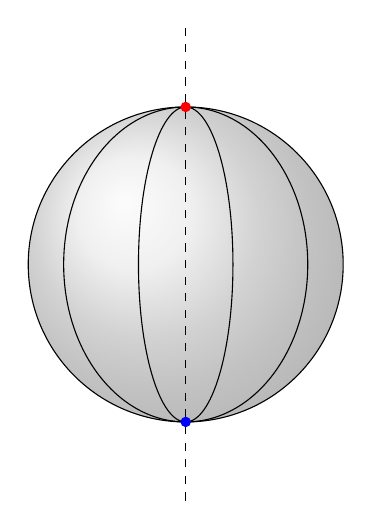
\begin{tikzpicture}
        \shade[ball color = gray!40, opacity = 0.4] (0,0) circle (2cm); % background colour grey
        \draw (0,0) circle (2cm); % draw outside of sphere
        \draw[dashed] (0,-3) -- (0,3);
        \draw (0,-2) arc (90:270:0.6 and -2); % second from left
        \draw (0,-2) arc (90:270:-0.6 and -2); % second from right
        \draw (0,-2) arc (90:270:1.55 and -2); % left half-meridian
        \draw (0,-2) arc (90:270:-1.55 and -2); % right half-meridian
        \draw (0,-2) node[fill=blue,shape=circle,scale=0.4]{}; % one 0-cell
        \draw (0,2) node[fill=red,shape=circle,scale=0.4]{}; % the other 0-cell
      \end{tikzpicture}
      \caption{The $C_n$-CW structure on $S^2$ with action by rotation around a vertical axis, shown here for $n = 8$. The two 0-cells are in blue and red, the 1-cell is in black, and the 2-cell is in grey.}
      \label{fig: rep sphere cyclic rotation}
\end{figure}

\begin{example}[Antipodal $C_2$-action on $S^2$]
    $S^2$ has another $C_2$-action, the antipodal one. Thinking of $S^2$ as a $C_2$-space in this new way, we get a different $C_2$-CW structure. It has:
    \begin{itemize}
        \item one 0-cell, of the form $C_2/e \times *$, corresponding to the orbit of a single point (i.e. some point together with its antipode);
        \item one 1-cell, attached at both ends to the 0-cell, of the form $C_2/e \times I$, forming both halves of a meridian;
        \item one 2-cell, attached to the one-cell, of the form $C_2/e \times D^2$, forming both hemispheres.
      \end{itemize}
      This $C_2$-action has no fixed points, and so the isotropy group of our 0-cell is different from that in the previous example. In fact, this $C_2$-space cannot be realised as (is not weak equivalent to) a representation sphere, because every representation sphere has at least an $S^0$ worth of fixed points, realised by $0$ and $\infty$.
\end{example}

\begin{example}[$S^1$-action on the torus]
    $G = S^1$ acts on the torus $S^1 \times S^1$ by rotation in the first factor. This action has no fixed points, and we get an $S^1$-CW structure with
    \begin{itemize}
        \item one 0-cell, of the form $S^1/e \times *$;
        \item one 1-cell, attached at both ends to the 0-cell, of the form $S^1/e \times I$.
      \end{itemize}
      Since the torus is $2$-dimensional and $S^1$ is $1$-dimensional, we should not be surprised that we required only 0- and 1- cells here. Topologically, the 0-cell is embedded as $S^1 \times * \subset S^1 \times S^1$ and the 1-cell is the orbit of $* \times S^1$ under the $S^1$-action. 
\end{example}

\begin{example}[$D_6$-action on a triangle]
    Let $T$ be a solid equilateral triangle in the plane. Then the dihedral group $D_6$ acts on $T$ by reflections and rotations. The corresponding $D_6$-CW structure has
    \begin{itemize}
        \item three 0-cells:
        \begin{itemize}
            \item the centre of $T$ is a fixed point, $D_6/D_6 \times *$;
            \item the three vertices of $T$ are an orbit, where each vertex is stabilised by a reflection, so this 0-cell has the form $D_6/C_2 \times *$;
            \item the three midpoints of edges of $T$ form a $0$-cell, $D_6/C_2 \times *$;
        \end{itemize}
        \item three 1-cells:
        \begin{itemize}
            \item the three line segments from a vertex to the centre of $T$ are each stabilised by a reflection, forming a cell $D_6/C_2 \times I$;
            \item the three line segments from the centre to the midpoint of an edge are also a $D_6/C_2 \times I$;
            \item the 6 line segments from a vertex to the midpoint of an edge form a free orbit $D_6/e \times I$;
        \end{itemize}
        \item one 2-cell: $T$ with the 0- and 1- cells described above removed is a free orbit (6 connected components), $D_6/e \times D^2$.
    \end{itemize}
    See Figure \ref{fig: triangle example} for a diagram.
\end{example}

\begin{figure}
    \centering
    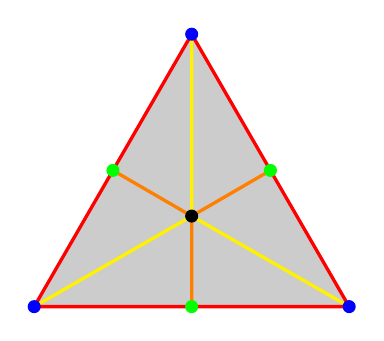
\begin{tikzpicture}[every node/.style={shape=circle,scale=0.5}]
        \fill[gray!40] (0,0) -- (4,0) -- (2,3.46) -- cycle; % fill triangle with grey
        \draw[very thick,yellow] (0,0) -- (2,1.15) % join vertices to centre
        (4, 0) -- (2,1.15) -- (2,3.46);
        \draw[very thick,red] (0,0) node[fill=blue]{} % outside edges and vertices
        -- (4, 0) node[fill=blue]{}
        -- (2,3.46) node[fill=blue]{} % top vertex has height 1/2 * base * sqrt{3}
        -- cycle;
        \draw[very thick,orange] (1,1.73) node[fill=green]{} % middle of edge to centre
        -- (2,1.15) node[fill=black]{} % centre node has height 1/2 * base * tan(pi/6)
        -- (3,1.73) node[fill=green]{}
        (2,0) node[fill=green]{} -- (2,1.15);
    \end{tikzpicture}
    \caption{The $D_6$-equivariant CW structure on a solid triangle. Each cell is in a single colour. The 2-cell consists of the 6 grey triangles.}
    \label{fig: triangle example}
\end{figure}

\section{The orbit category and Elmendorf's Theorem}

In addition to the Whitehead Theorem, $G$-CW complexes have other nice properties. One important such is that taking $H$-fixed points commutes with the construction of $G$-CW complexes (although the $H$-fixed points functor does not commute with colimits in general). Remember, if we hope to understand weak equivalences then we need to understand how to take $H$-fixed points.

\begin{prop} The functor $(-)^H$ commutes with 
    \begin{itemize}
        \item pushouts where one map is a closed inclusion, and
        \item sequential colimits along closed inclusions.
    \end{itemize}
    In particular, $(-)^H$ commutes through the construction of a $G$-CW complex. 
\end{prop}

To understand the $H$-fixed points of a $G$-space given some $G$-CW structure, it is thus sufficient to understand the $H$-fixed points of each cell separately. Doing so amounts to computing 
\[(G/K \times D^n)^H = (G/K)^H \times D^n = \Map^G(G/H, G/K) \times D^n\]
so we really only need to understand fixed points of the form 
\[(G/K)^H = \Map^G(G/H, G/K).\] 
We can package up all the mapping spaces we need into a convenient form, called the orbit category.

\begin{defn}[Orbit category]
    The orbit category $\O_G$ is the full subcategory of $\GTop$ on the objects $G/H$.
\end{defn}

Mapping spaces in the orbit category have the form $\Map^G(G/H, G/K)$, which we want to understand. We claim that such maps correspond to elements $g \in G$ producing subconjugacy relations $gHg^{-1} \subseteq K$. A $G$-equivariant map $f: G/H \to G/K$ is completely specified by where it sends the identity coset $eH$. Taking $f(eH) = gK$, we get the relation 
\[hgK = hf(eH) = f(heH) = f(eH) = gK\]
for every $h \in H$, which is equivalent to requiring $g^{-1}Hg \subseteq K$. Two maps corresponding to subconjugacy relations $g_1^{-1}Hg_1 \subseteq K$ and $g_2^{-1}Hg_2 \subseteq K$ are the same if $g_1K = g_2K$.

Before discussing some examples of orbit categories, we state the main result which explains why we care about them. 

\begin{thm}[Elmendorf]\label{thm: Elmendorf}
    The functor 
    \begin{align*} \Psi: \GTop &\to \Fun(\O_G^{\op}, \Top)\\
            X &\mapsto (G/H \mapsto X^H) 
    \end{align*}
    induces an equivalence of $\infty$-categories. 
\end{thm}

The point of Elmendorf's Theorem, for us, is that presheaves on the orbit category gives a very concrete $\infty$-categorical model for $\GTop$. To think of $\GTop$ as an $\infty$-category another way, we localize at the $G$-weak equivalences, and while this is formally easy to do, it can be hard to get one's hands on the result. The orbit category itself is easy to access, and this model of $\GTop$ as presheaves on the orbit category is the one we want to use going forwards. 

\begin{remark}
    If you are uncomfortable with the language of $\infty$-categories, you should think of Elmendorf's Theorem as saying that the homotopy theory of $G$-spaces up to $G$-weak equivalence is the same as the homotopy theory of presheaves on the orbit category, up to pointwise weak equivalence of topological spaces. Explicitly, this means that:
    \begin{itemize}
        \item homotopy limits and colimits behave the same, and
        \item the homotopy categories on the left and right are the same.
    \end{itemize}
    Another way to think about this result is that as 1-categories, it's easy to see that the left and right sides encode the same data. But the $\infty$-categorical structure on the right turns out to be technically much easier to work with, so we prefer to use it. Elmendorf's Theorem tells us we are allowed to do this, since we will get the same notion of weak equivalence either way.
\end{remark}

\begin{remark}
    The equivalence in Elmendorf's Theorem comes from an adjunction, with $\Psi$ being right adjoint to evaluation at $G/e$.
\end{remark}

Next we will see three examples of orbit categories. 

\begin{example}[$\O_*$]
    Take $G = *$, then $\O_*$ has a single object called $*/*$ with unique endomorphism the identity. A presheaf on this orbit category is just a topological space $X$, so what Elmendorf's Theorem is saying in this case is that the category of $G$-spaces for $G = *$ is equivalent to $\Top$ itself, and a $*$-weak equivalence is the same as a topological weak equivalence.
\end{example}

\begin{example}[$\O_{C_2}$] Let $G = C_2$. Then the orbit category $\O_{C_2}$ has two objects, $C_2/e$ and $C_2/C_2$. Since $G$ is abelian, asking for a subconjugacy relation $gHg^{-1} \subseteq K$ is the same as asking for $H \subseteq K$, in which case we get $C_2/K$ distinct maps. We have 
    \[\Map^{C_2}(C_2/e, C_2/e) = C_2, \Map^{C_2}(C_2/C_2, C_2/C_2) = \Map^{C_2}(C_2/e, C_2/C_2) = \{e\},\]
    while $\Map^{C_2}(C_2/C_2, C_2/e) = \emptyset$. We can depict this orbit category as 
    \[\begin{tikzcd}
        C_2/e \arrow[r] \arrow[loop, distance=2em, in=305, out=235] \arrow[loop, distance=2em, in=125, out=55] & C_2/C_2 \arrow[loop, distance=2em, in=305, out=235]
        \end{tikzcd}\]
    with a unique non-identity endomorphism of the non-terminal object $C_2/e$.
\end{example}

\begin{example}[$\O_{C_{2^n}}$]\label{ex: orbit of C2n}
    Let $G = C_{2^n}$. Then $G$ has precisely one cyclic subgroup of size $2^k$ for each $0 \leq k \leq n$, and the poset of subgroup inclusions is totally ordered by size. Again $G$ is abelian, so we compute 
    \[|\Map^G(C_{2^n}/C_{2^k}, C_{2^n}/C_{2^l})| = \begin{cases} 2^{n-l} & k \leq l \\ 0 & k > l. \end{cases}\] 
    The orbit category looks like
    \[\begin{tikzcd}
    C_{2^n}/e \arrow[r] \arrow[loop, distance=2em, in=305, out=235] & \ldots \arrow[r] & C_{2^n}/C_{2^k} \arrow[r] \arrow[loop, distance=2em, in=305, out=235] & C_{2^n}/C_{2^{k+1}} \arrow[loop, distance=2em, in=305, out=235] \arrow[r] & \ldots \arrow[r] & C_{2^n}/C_{2^n} \arrow[loop, distance=2em, in=305, out=235]
    \end{tikzcd}\]
    with an arrow whose codomain is $C_{2^n}/C_{2^k}$ representing $2^{n-k}$ distinct maps. 
\end{example}

\section{Equivariance in families}

Thus far, we have made many statements which we required to hold for all closed subgroups $H$ of $G$. Do we really always need to work with \emph{all} closed subgroups? What if we wanted to restrict to finite subgroups, or finite-index subgroups? Of course, if we redefine $G$-CW complexes and $G$-weak equivalences in terms of some restricted collection of subgroups of $G$, we will get a different homotopy theory. Nonetheless, Elmendorf's Theorem holds for such families.

\begin{defn} A family $\F$ of subgroups of $G$ means a collection of subgroups closed under conjugation and taking subgroups (i.e. closed under subconjugacy relations).
\end{defn}

Given a family of subgroups $\F$, we get induced homotopy theories on both sides of Elmendorf's Theorem.
\begin{itemize}
    \item In $\GTop$, a map $f: X \to Y$ is a weak equivalence if $f^H: X^H \to Y^H$ is a (topological) weak equivalence for all subgroups $H \in \F$. 
    \item In $\Fun(\O_G^{\op}, \Top)$, a weak equivalence is a map which is pointwise a topological weak equivalence, at all points $G/H$ where $H \in \F$. 
\end{itemize}

\begin{example}
    If we take $\F$ to be the collection of all subgroups of $G$, we recover the notion of $G$-weak equivalence defined previously. If we take $\F = \{e\}$ to only contain the identity subgroup, we get Borel weak equivalence. In between these extremes, one might let $\F$ be the set of all finite subgroups of $G$.
\end{example}

In particular, if $G = S^1$ one often wants to consider the family of finite subgroups, since fixed points under the $C_n$-action are often more easily understood than $S^1$-fixed points. 

\begin{remark}
    Elmendorf's theorem is still true if we use some family $\F$ to specify the weak equivalences on both sides. 
\end{remark}

\begin{example}[Families in $C_{2^n}$]
    Consider again Example \ref{ex: orbit of C2n}. Since a family must be closed under taking subgroups, a family in $C_{2^n}$ amounts to a choice of maximal subgroup $C_{2^k}$, and has the form $\F = \{e, C_2, \ldots, C_{2^k}\}$. Then restricting from all subgroups of $C_{2^n}$ to the family $\F$ is not the same as applying the forgetful functor from $C_{2^n}$-spaces to $C_{2^k}$-spaces, because in the former case we retain a residual Borel-equivariant $C_{2^n}$-action. 
\end{example}

\begin{remark}
    Elmendorf's Theorem for a specific choice of family $\F$ will come up later in the seminar, when we talk about isotropy separation and the slice spectral sequence. 
\end{remark}

\printbibliography

\end{document}